\chapter*{Introduction}
\addtocontents{toc}{\protect\vspace{\beforebibskip}} % to have the bib a bit from the rest in the toc
\addcontentsline{toc}{chapter}{\tocEntry{Introduction}}

\renewcommand{\thefigure}{\Alph{figure}}

\epigraph{
pity this busy monster, manunkind,
    }{
    --- \textsc{E. E. Cummings}}

\epigraph{
[...] og fordi jeg alltid har hatt en dragning mot det skjulte og hemmelige.
    }{
    --- \textsc{K. O. Knausgård}, \textit{Om Høsten}}

\begin{figure}[tb]
\centering
\scalebox{0.8}{%Angle Definitions
%-----------------

%set the plot display orientation
%synatax: \tdplotsetdisplay{\theta_d}{\phi_d}
\tdplotsetmaincoords{60}{110}

%define polar coordinates for some vector
%TODO: look into using 3d spherical coordinate system
\pgfmathsetmacro{\rvec}{.8}
\pgfmathsetmacro{\thetavec}{30}
\pgfmathsetmacro{\phivec}{60}

%start tikz picture, and use the tdplot_main_coords style to implement the display 
%coordinate transformation provided by 3dplot
\begin{tikzpicture}[scale=5,tdplot_main_coords]

%set up some coordinates 
%-----------------------
\coordinate (O) at (0,0,0);

%determine a coordinate (P) using (r,\theta,\phi) coordinates.  This command
%also determines (Pxy), (Pxz), and (Pyz): the xy-, xz-, and yz-projections
%of the point (P).
%syntax: \tdplotsetcoord{Coordinate name without parentheses}{r}{\theta}{\phi}
\tdplotsetcoord{P}{\rvec}{\thetavec}{\phivec}

%draw figure contents
%--------------------
% HAMILTONIAN AXIS
\draw[thick,->] (0,0,0) -- (1.5,0,0) node[anchor=north east]{Hamiltonian $(\begingroup\color{brewerRed}{y}\endgroup)$};
\draw (1/3, .01pt, 0pt) -- (1/3, -.04pt, 0pt) node[anchor=east] {\begingroup\color{brewerRed}{one-component}\endgroup};
\draw (2/3, .01pt, 0pt) -- (2/3, -.05pt, 0pt) node[anchor=east] {\begingroup\color{brewerRed}{two-component}\endgroup};
\draw (1, .01pt, 0pt) -- (1, -.05pt, 0pt) node[anchor=east] {\begingroup\color{brewerRed}{four-component}\endgroup};

% BASIS AXIS
\draw[thick,->] (0,0,0) -- (0,1.5,0) node[anchor=north west]{Basis $(\begingroup\color{brewerYellow}{M}\endgroup)$};
\draw (0pt, 1/3, -.01pt) -- (0pt, 1/3, +.05pt) node[anchor=south] {\begingroup\color{brewerYellow}{double zeta}\endgroup};
\draw (0pt, 2/3, .01pt) -- (0pt, 2/3, -.05pt) node[anchor=north] {\begingroup\color{brewerYellow}{triple zeta}\endgroup};
\draw (0pt, 1, -.01pt) -- (0pt, 1, +.05pt) node[anchor=south] {\begingroup\color{brewerYellow}{quadruple zeta}\endgroup};

% METHOD AXIS
\draw[thick,->] (0,0,0) -- (0,0,1.5) node[anchor=south]{Method $(\begingroup\color{brewerBlue}{x}\endgroup)$};
\draw (0pt, .01pt, 1/3) -- (0pt, -.05pt, 1/3) node[anchor=east] {\begingroup\color{brewerBlue}{Hartree--Fock}\endgroup};
\draw (0pt, .01pt, 2/3) -- (0pt, -.05pt, 2/3) node[anchor=east] {\begingroup\color{brewerBlue}{MP2}\endgroup};
\draw (0pt, .01pt, 1) -- (0pt, -.05pt, 1) node[anchor=east] {\begingroup\color{brewerBlue}{CCSD(T)}\endgroup};

\end{tikzpicture}
}
\caption{The three dimensions of Relativistic Quantum Chemistry. The computational scaling of a relativistic model chemistry is
$ S=\textcolor{red}{y}(\textcolor{blue}{x})f(\textcolor{blue}{x})\textcolor{green}{M}^{\textcolor{blue}{x}} $. The expense of relativity is in
the appearance of a new prefactor, not in the $M$-dependence of the particular method.}
\label{fig:RQC-axis}
\end{figure}
and look at different axes.

\section*{What Are the Electrons Really Doing in Molecules?}

\todo[inline]{Write something about the scope of molecular quantum
mechanics.}

This question was posed by R.~S.~Mulliken over a half-century ago, as
lecture title for the acceptance of the Gilbert N.~Lewis award in 1960.

This will be the subject of Chapter \ref{ch:QM}

\section*{The Problem of Solvation or Taming Complexity with Models}

Chemistry can be largely considered a \emph{wet} science: almost always
chemical phenomena happen in a liquid environment.~\autocite{Reichardt2010-le}
We hereby define a "solution", or more generally an "environment", as
a system were the number of solvent molecules exceeds by far the number
of solute molecules.~\autocite{Tomasi2004-dc, Tomasi2007-es}
It is then clear that theoretical and computational approaches to such a
problem will necessarily suffer from a \emph{dimensionality disease}.
The number of degrees of freedom to be taken into account is, in
principle, so large, that even the most advanced computing machines
would have a hard time computing the desired observables.
Moreover, on an interpretive level, it would not even be desirable to
have such a detailed insight.
As is well known from statistical mechanics, microscopic detail cannot
account for the macroscopic behaviour.~\autocite{Hill1960-ql,
Hansen2013-io}
To tame this complexity and cure the disease, one must devise
\emph{models} that simplify physical reality, while offering tools for
understanding reality and predicting new and exciting
phenomena.~\autocite{Anderson1972-ai, Winsberg2010-sy, Kovac2011-ew}
One of the earlier attempts at tackling the problem of solvation is due
to \citeauthor{Onsager1936-wf}. His was a rather crude model, but one
that has had a lasting impact and informs much of the developments that
will be presented in this thesis.~\autocite{Onsager1936-wf}

Before introducing our model of choice, let us consider how an
environment might affect molecular observables of interest.
Environment effects are usually classified as:
\begin{itemize}
\item \emph{direct}.
  These effect stem straightforwardly from the modification underwent by
  the solute electronic density when interacting with the environment.
\item \emph{Indirect}.
  It is common for solutes to exhibit different minimum-energy
  conformations in different environments. These effects are commonly
  labelled as indirect.
\item \emph{Local field}.
  Light-matter interactions are also affected by the environment. Local
  modifications of externally applied fields subtly influence molecular
  responses.~\autocite{Cammi1998-jp, Pipolo2014-sd}
\item \emph{Dynamic}.
  Probing the nature of molecular excited states has enormous
  technological impact. The presence of the environment radically
  influences excited states, since relaxation processes in the medium
  become important.
\item \emph{Specific}. This catch-all category includes all effects
  stemming from the peculiar solute-solvent pair interactions that
  cannot be fully described under any of the previous labels.
  In general, modelling such effects demands an atomistic level of
  detail.
\end{itemize}

Faced with the problem of describing such a diverse array of effects,
two main models have emerged in the past decades, each with its
strengths and weaknesses.
Both can be classified as \emph{multiscale} (or \emph{focused})
models~\autocite{Nobel2013} and hinge on the same idea: treat different
parts of the system with different methods and couple these methods by
bridging "scales" at the boundary, \emph{vide infra}.
While both models treat the molecular degrees of freedom at the quantum
mechanical level, their approach to the microscopic description of the
degrees of freedom of the environment differs:
\begin{itemize}
 \item
   \emph{Discrete} (or \emph{explicit}) models explicitly treat those
   degrees of freedom.
   This is either achieved by a cheaper quantum mechanical
   method~\autocite{Vreven2006-gx} or by \ac{MM}.~\autocite{Senn2009-sk}
   In the latter approach, commonly dubbed \acs{QM}/\acs{MM}, the \acs{MM}
   region can either be polarizable~\autocite{MMPol} or non
   polarizable.~\autocite{MM}
 \item
   \emph{Continuum} (or \emph{implicit}) completely remove the degrees
   of freedom of the environment from the picture, replacing it with a
   structureless continuum.
   The effect of this continuum is described, classically, \emph{via}
   its bulk properties.~\autocite{Onsager1936-wf, Miertus1981-mm}
\end{itemize}
\acs{QM}/\acs{MM} models can capture, albeit approximately, the effect
of the atomistic nature of the environment on the active part of the
system.
However, they demand a statistical average of environment configurations
to yield results of any significance. Moreover, a large number
\emph{cutoff} for the \acs{MM} region is usually required to converge
long-range electrostatic interactions.~\autocite{Something here??}
Continuum models avoid both problems at once. Statistical averaging is
built into the model \emph{via} their parametrization by
means of the environment's bulk properties, such as the permittivity.
In addition, long-range electrostatics is treated exactly.
Unfortunately, atomistic detail is lost and it is then impossible to
recover a satisfactory description of specific effects.
To partly alleviate these sources of error, the \acs{QM}/\acs{MM} and
\acs{QM}/Continuum methods can and have been successfully combined to
yield the three-layer \acs{QM}/\acs{MM}/Continuum method.~\autocite{Curutchet, Steindal Lipparini}
Figure \ref{fig:qm-to-multiscale} schematically portrays the transition
from a full \acs{QM} model of the relevant system to its multiscale
representations.

\begin{figure}[tb]
\missingfigure{Add picture with multiscale models}
\caption{From quantum mechanical models to multiscale models.}
\label{fig:qm-to-multiscale}
\end{figure}

Notice that we have deliberately ruled out so-called \emph{cluster}
models from the above discussion.~\autocite{ClusterModels}
These approaches replace the actual physical setting with a suitable
truncation of the whole solute+solvent system, the \emph{model system}
and treat it within a chosen quantum mechanical level of theory.
Cluster models can be used to benchmark more approximate multiscale
models, but their description is outside the scope of this thesis.

Chapter \ref{ch:CSM} will present an overview of the \ac{PCM} for
solvation.
I will present a nontechnical discussion of the mathematical details of
the model and an outline of current methodologies for the solution of
the associated governing equations.
Borrowing from the work of \citeauthor{Lipparini2010-be},\autocite{Lipparini2010-be,
Lipparini2015-lq} I will introduce a unifying theoretical formalism for
\acs{QM}/Continuum, \acs{QM}/\acs{MM} and \acs{QM}/\acs{MM}/Continuum models that will
be extensively used throughout the thesis.

\todo[inline]{CURRENTLY VERBATIM FROM MASTER THESIS}

Continuum models arise as limits, in a proper sense, to the discrete
models. To stress this point we introduce the \emph{solution}
Hamiltonian in the Born--Oppenheimer approximation as:
\begin{equation}\label{eq:solution-ham}
 H(\vect{r}_\mathrm{M}, \vect{r}_\mathrm{S}) =
  H_\mathrm{M}(\vect{r}_\mathrm{M}) +  H_\mathrm{S}(\vect{r}_\mathrm{S})
+ H_\mathrm{MS}(\vect{r}_\mathrm{M}, \vect{r}_\mathrm{S})
\end{equation}
where the subscript M refers to the solute while S to the solvent. The
coordinates $(\vect{r}_\mathrm{M}, \vect{r}_\mathrm{S})$ refer to
\emph{both} nuclei and electrons, the interaction term is given by the
usual Coulombic electrostatic Hamiltonian.

It is important to remark that nuclear coordinates must be considered
explicitly. Liquid phases are, by definition, characterized by the high
mobility of their molecular constituents. Changes in the internal
geometry of solvent molecules, triggered by intermolecular interactions
between themselves and with the solute, always play a role in the
solvation process. Whether this role is prominent or not cannot be
decided \emph{a priori}.

From a computational point of view, using the Hamiltonian in Eq.~\eqref{eq:solution-ham} is simply not feasible. We would have to
determine a \acs{PES} of enormous dimensionality and then explore the full
dynamics of the system. Even assuming that the minimum energy
conformation on the \acs{PES} can be fully characterized, its knowledge will
not lead us to a correct description of the physics of solvation. In
fact, macroscopic observables of systems with a large number of degrees
of freedom arise as \emph{average} values of the microscopic behaviour
of every single component, the average being either on the phase space
trajectory or on the appropriate ensemble.~\autocite{Hill1960-ql}. It is always
necessary to perform some kind of average upon the energies
corresponding to all the accessible conformations of the whole
solute+solvent system.

Of course, this formidable task may be accomplished using statistical
thermodynamics and the idea of \emph{statistical ensembles} developed by
Gibbs. To apply the idea of an ensemble average we must resort to a
molecular dynamics or Monte Carlo simulation of the solution, in order
to obtain the appropriate partition function, $Z$. This introduces a
number of points that will be central in the development of continuum
models:
\begin{enumerate}
 \item statistical simulations rely on \emph{macroscopic} parameters
   such as the temperature or the density. These parameters are not
   present in the Hamiltonian \eqref{eq:solution-ham}, but are necessary
   for the description of molecular systems in the condensed phase. This
   is true whether one considers discrete or continuum approaches;
 \item the basic energetic quantity is the thermodynamic potential
   characterizing the chosen ensemble. If a direct comparison with the
   experiment is sought, one should run a simulation in the $(NpT)$
   ensemble whose potential is the Gibbs free energy $G$. This point is
   of paramount importance in continuum models and we will have the
   opportunity to stress it in this Chapter as well as in Chapter
   \ref{chap:relpcmscf};
 \item even starting from a completely atomistic point of view, our
   final results will always be in the form of an average over solvent
   conformations. We have explicitly replaced a discrete description
   with a continuous distribution function. Atomistic details can of
   course be recovered by further analysis, but the point remains:
   properties of solutions (the solvation energy among them) have an
   intrinsic average nature.
\end{enumerate}

The fact that an averaging procedure is essential in studying solvation
processes should convince the reader that, at least from a purely
mathematical point of view, we can replace the full Hamiltonian
\eqref{eq:solution-ham} with an \emph{effective} Hamiltonian, averaging
the solvent degrees of freedom in a preliminary
step.~\autocite{Angyan1992-vo, Tapia1992-pu}
\todo[inline]{Some pieces missing here, FILL IN}
Alternatively, an approximate decoupling can be obtained replacing the
mean-field operator in Eq.~\eqref{eq:ave1} by its classical average over
a suitable ensemble:
\begin{equation}\label{eq:ave_classic}
 \Braket{H_\mathrm{MS}}_\mathrm{S} = \frac{\int\diff\Gamma H_\mathrm{MS}\exp
\left(-\beta H_\mathrm{S}\right)}{\int\diff\Gamma\exp\left(-\beta H_\mathrm{S}\right)}.
\end{equation}
This classical average can be written in terms of the $g(\vect{r})$ distribution functions. These functions are defined
for the electrons and the nuclei of the solvent with respect to the fixed frame of reference of the solute molecule, see \noparcite[ref.][]{hansen}.
This amounts to considering the solvent as a structureless continuum, hence defining continuum models.

Continuum models are then characterized, by a solute-only
\emph{effective} Hamiltonian:\footnote{We will use the symbol
$H_\mathrm{MS}$ for the interaction Hamiltonian even if it is not the
full interaction term of Eq.~\eqref{eq:solution-ham}.}
\begin{equation}\label{eq:effective-ham}
 H(\vect{r}_\mathrm{M}) = H_\mathrm{M}(\vect{r}_\mathrm{M})
+ H_\mathrm{MS}(\vect{r}_\mathrm{M}),
\end{equation}
the explicit form of the averaged interaction in
Eq.~\eqref{eq:effective-ham} is in terms of solvent \emph{response
functions}, $Q_x(\vect{r},\vect{r}^\prime)$.
As will be apparent in the following, this term may depend on the solute
density, making the effective Hamiltonian \emph{nonlinear}.

An hierarchy of approximations for the resolution of the effective
Schr\"odinger equation can be devised, as was done for the discrete
models. The distinguishing feature is now the \emph{order} of the
solvent response functions used in the definition of the interaction
term.

If we limit ourselves to a linear response of the solvent we obtain the
class of models commonly called continuum solvation models, the
Polarizable Continuum Model among them. Computer simulations can be used
to determine these functions, but almost always one uses bulk properties
of the pure solvent obtained from experiment.

This, at first sight, crude approximation is rather well justified by
the following argument: from a physical point of view, our solution is
extremely dilute. The presence of the solute is an extremely small
perturbation for the bulk of the solvent and it is safe to assume that
the macroscopic properties of the solution are not far from those of the
pure solvent. Furthermore, the use of macroscopic experimental values
implicitly takes into account the averaging procedure one would carry
out in atomistic simulations of the solution.

As pictorially represented in Figure \ref{fig:discretetocontinuum} the
solvent is now a \emph{structureless polarizable} continuum and the
solute is accommodated inside a cavity formed in this continuum.
\begin{figure}[!h]
 \centering
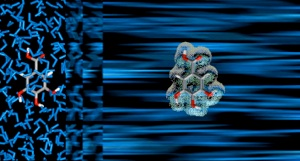
\includegraphics[width=.5\textwidth]{discretetocontinuum}
\caption{Pictorial representation of the transition from a discrete to a
continuum model of a solution.}
\label{fig:discretetocontinuum}
\end{figure}

\section*{The Road to Reality or Molecular Response Properties}

Characterizing, explaining and predicting the effect of the chemical
environment on a large number of measurable properties requires,
however, a synergistic experimental and theoretical approach.

This will be the subject of Chapter \ref{ch:molprop}

\section*{Accurate Methods for Accurate Properties}

This will be the subject of Chapter \ref{ch:solvation-correlation}
